\subsection{Physics of the Static Field}
\label{sec:PhyField}
% 1. - Main Magnet                                   [🔴 High Priority]
%      (Primary source of static magnetic field and spatial gradients.)

Electric current flowing through a wire coil generates a magnetic field, and is the fundamental physical principle of the MR system. Field strength, temporal stability, and homogeneity are used to evaluate system performance. Clinical \gls{mri} main magnets are typically made of superconducting wire-wrapped cylinders. These wires are made from niobium-titanium alloys and show no resistance to electric current when maintained at extremely low temperatures and align the field along the patient's cranial-caudal axis \cite{Prince_MedicalImaging_2015}. 

The amplitude of the current $I$ and $n$, the turn density (turns per unit length), represent together the two quantities that determine the magnetic field strength magnitude for an ideal solenoid $B = \mu_{0} \, n I$. The field is directed along the solenoid's long axis. A good estimate of the magnetic field at position z along the bore axis, measured from the solenoid center,within a finite solenoid of length $L$ and radius $R$ can be calculated from Biot–Savart's law 

\begin{equation}
	B(z) = \frac{\mu_0 n I}{2} 
	\left[
	\frac{z + \frac{L}{2}}{\sqrt{R^2 + \left(z + \frac{L}{2}\right)^2}} 
	-
	\frac{z - \frac{L}{2}}{\sqrt{R^2 + \left(z - \frac{L}{2}\right)^2}}
	\right],
\end{equation}

\noindent where $\mu_0$ is the permeability of free space \cite{griffiths2013electrodynamics}. This formula provides the axial field along the solenoid, with the maximum occurring at the center ($z=0$) and decreasing smoothly toward the ends. A simulation of this model for a 1.4 $m$ length by 0.6 $m$ diameter ideal solenoid was used, to approximate a real \gls{mri} system, such as the Siemens Magnetom Trio\textsuperscript{\texttrademark}, used at \gls{bergan}.

Figure \ref{fig:Bz_vs_zSet} showcases this model in two parts. First, the magnetic field ($B_0$) along the z-axis, where $z=0$ corresponds to isocenter with dashed vertical lines and light blue shading marking the solenoid boundaries at z = $\pm$ 0.704 m away from isocenter. The field is normalized to a maximum of $B_0 = 3$~T, shown as a dashed horizontal reference line, with no shielding or distortion applied. 

\begin{figure}[htb!]
	\centering
	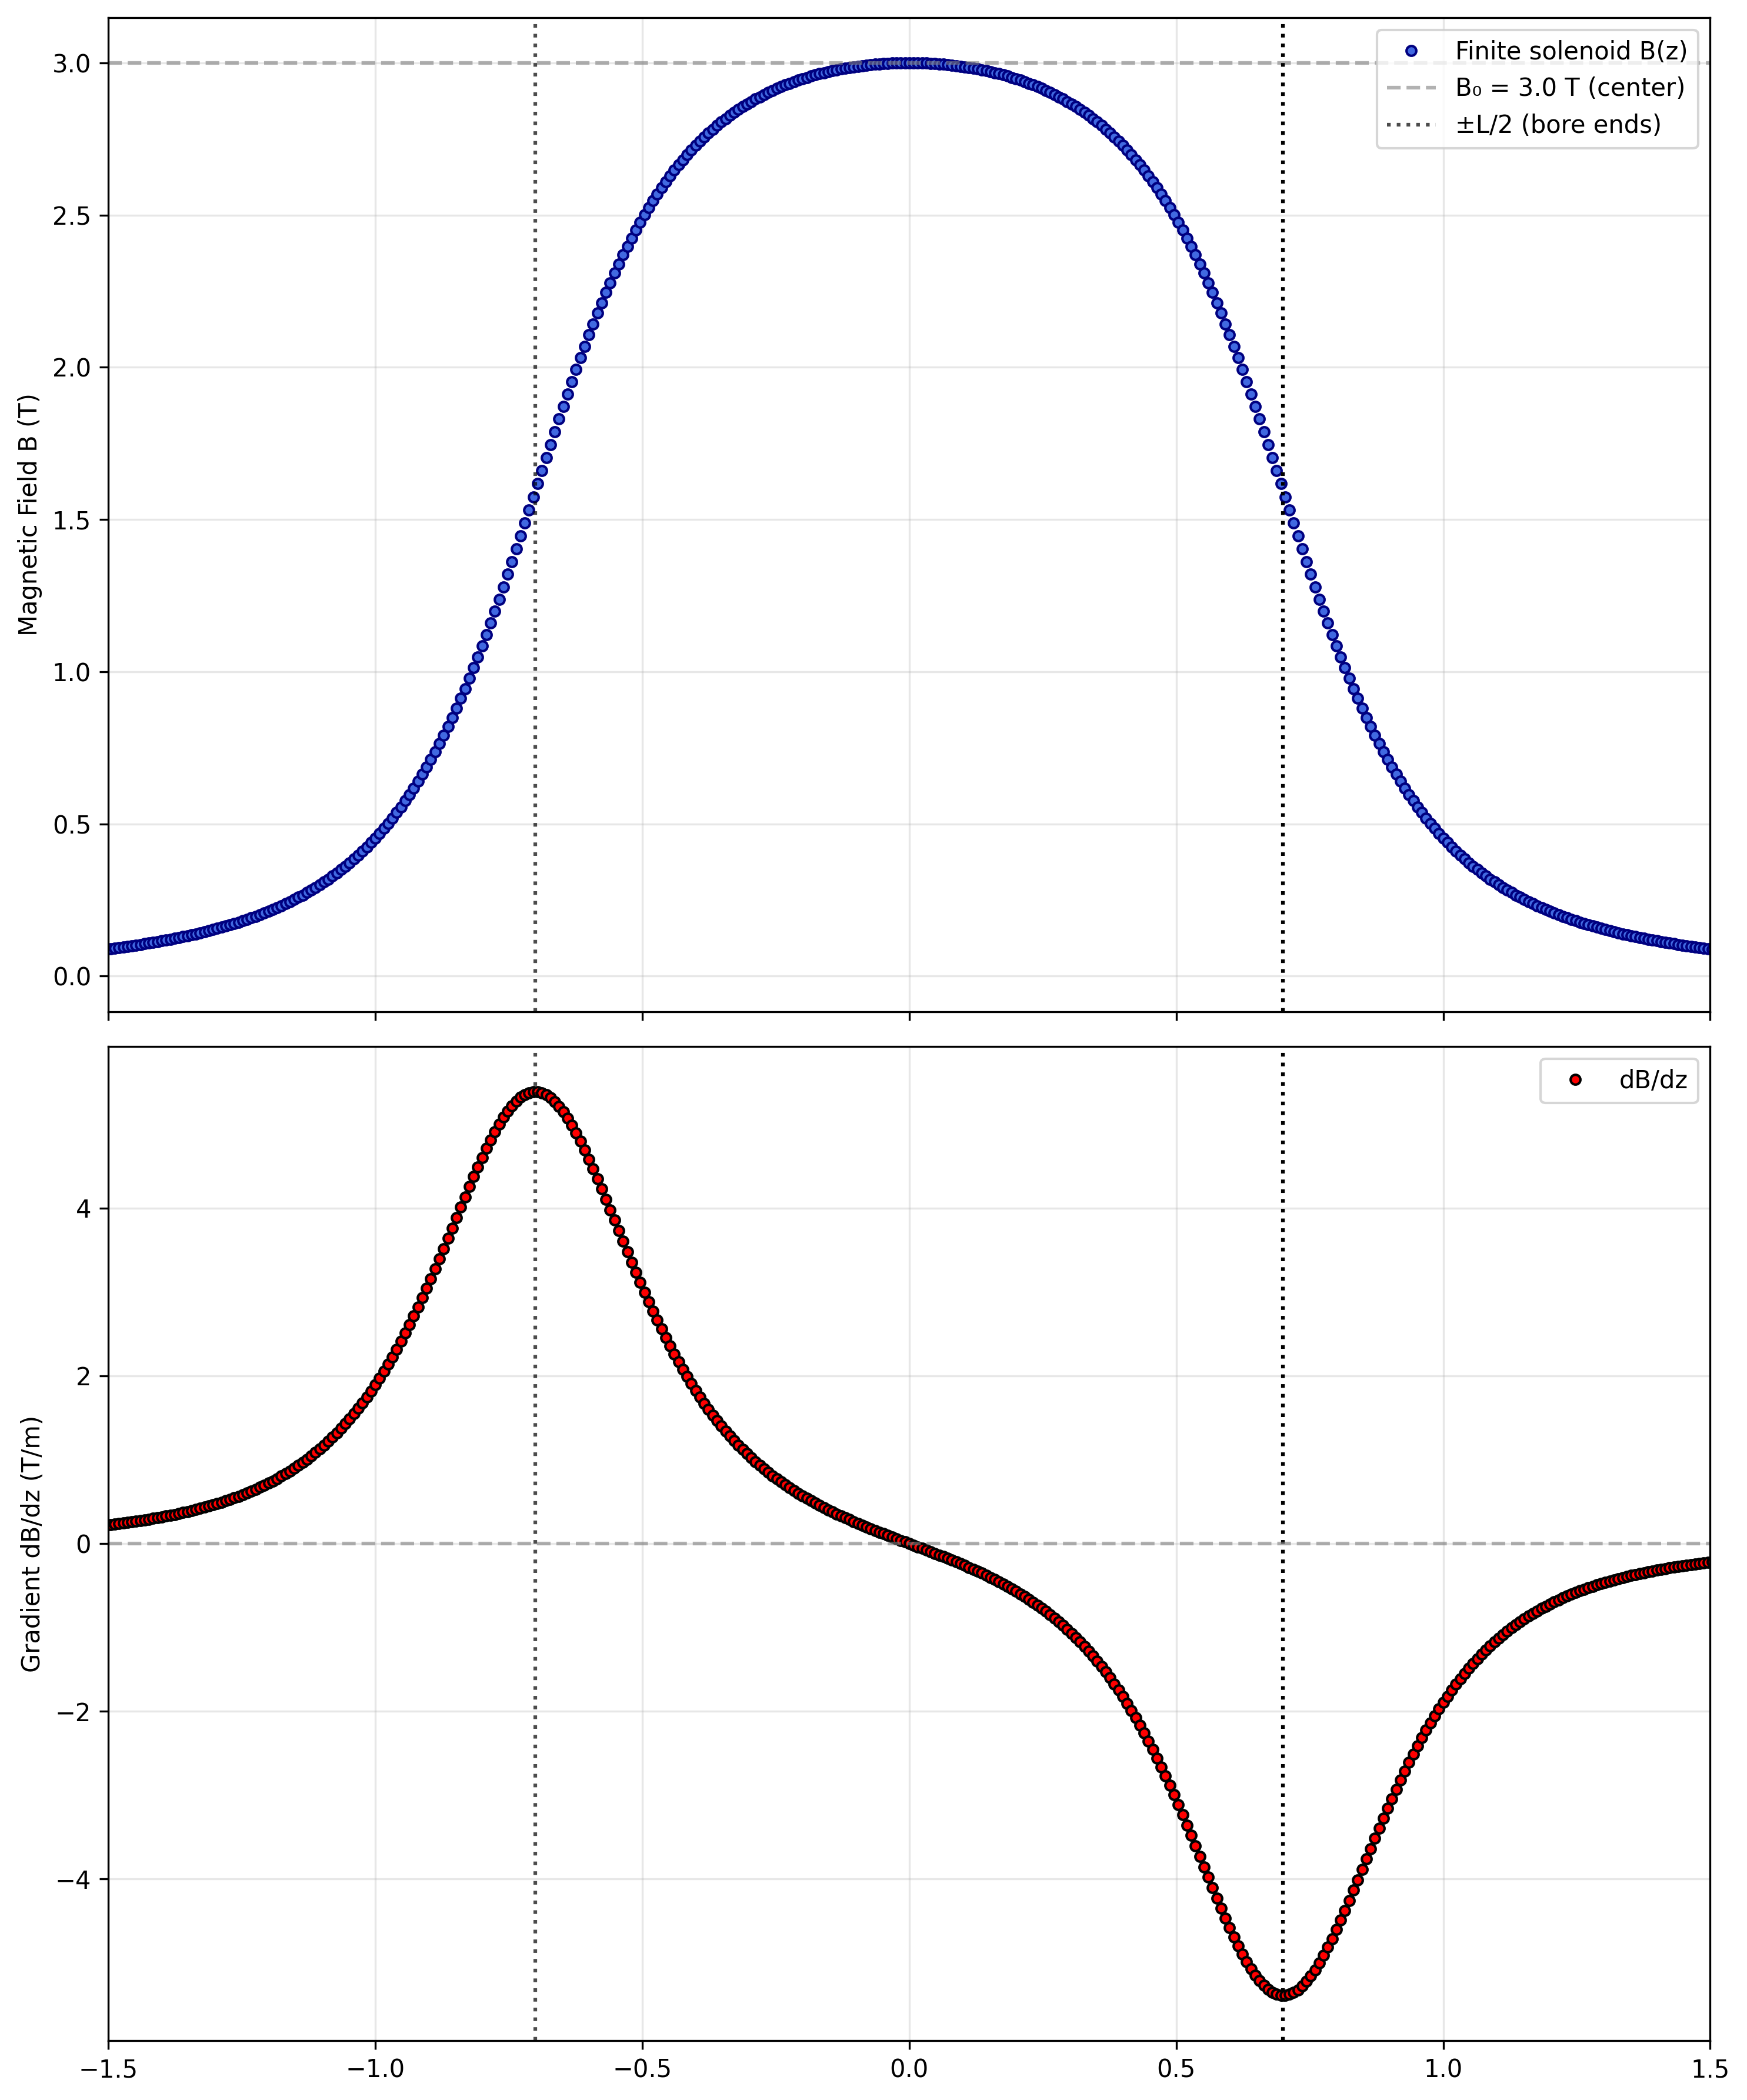
\includegraphics[width=0.65	\textwidth]{Assets/FieldMapping.png}
	\caption[Axial magnetic flux density $B_z$ and spatial gradient for an idealized 3 T MRI solenoid]{Axial magnetic flux density $B_z$ and spatial gradient for an idealized 3 T \gls{mri} solenoid (L = 1.4 $m$, R = 0.3 $m$). Top: The magnetic field peaks at 3T at the isocenter (z = 0 $m$) and decreases symmetrically toward both ends. Grey dotted lines indicate the solenoid edges (bore entrances). Bottom: The spatial gradient $dB_z/dz$ reaches its maximum magnitude at the bore entrances (z = ±0.704 $m$).}
	\label{fig:Bz_vs_zSet}
\end{figure}

Second, the axial field $B(z)$ from the finite solenoid model yields a spatial gradient $dB_z/dz$, its maximum value is confirmed to be at the bore entrance position \cite{astmF2052,ferreira2017} ($z \approx \pm 0.704$ m for this 1.4 m length example), as shown in the bottom panel of Figure \ref{fig:Bz_vs_zSet}. These strong gradients (often several T/m near entrances) exert attractive forces on paramagnetic/ferromagnetic objects (pulling toward higher $|B|$) and repulsive on diamagnetic ones (pushing away), posing projectile hazards \cite{bushberg2011,astmF2052,ferreira2017}. This gradient-driven behavior supports ASTM displacement force testing and motivates shielding designs in modern systems. High-susceptibility materials experience the strongest pull toward the isocenter, with the maximum risk at bore entrances.

Having established the spatial distribution of the static field, we now turn to how this field interacts with matter. These interactions are governed by fundamental electromagnetic theory and provide the foundation for classifying materials by magnetic susceptibility which quantifies \gls{mri} safety risks for implanted devices according to ASTM standards \cite{astmF2052,astm2213}.

\subsection{The Static Field interaction with matter}

Any material placed in a magnetic field develops a magnetization, $\mathbf{M}$, defined as the net magnetic dipole moment per unit volume, $\mathbf{M} \equiv \frac{\boldsymbol{m}}{V}$ \cite{griffiths2013electrodynamics}. In a way this  $\mathbf{M}$ represents a ``smoothed'' magnetization of an average field effect over many atoms. At the atomic level, the magnetic field inside a material fluctuates rapidly due to particles in motion. This phenomena forms the basis for \gls{mri} image generation. However, for the purpose of this thesis, we focus on the macroscopic behavior mostly. To simplify the macroscopic analysis of materials in magnetic fields, the auxiliary magnetic field $\mathbf{H} \equiv \frac{1}{\mu_0} \mathbf{B} - \mathbf{M}$, where $\mathbf{B}$ is the macroscopic magnetic flux density and $\mu_0$ is the permeability of free space, accounts for the contribution to the magnetic field from free currents, separating it from the contribution of bound currents induced by magnetization \cite{griffiths2013electrodynamics}. This distinction becomes useful when analyzing mechanical effects on magnetic dipoles.

Different materials respond differently to an applied field. For linear materials magnetization is also directly proportional to the field strength $\mathbf{M} = \chi_m \mathbf{H}$, the degree to which a material becomes magnetized is quantified by its magnetic susceptibility, $\chi_m$, which is typically around $-10^{-5}$ to 0 for biological tissues. It is convenient to define the material permeability as $\mu \equiv \mu_0(1 + \chi_m)$, so that the magnetic flux density takes the compact form

\begin{subequations}
	\begin{align}
		\mathbf{B} &= \mu_0(1+\chi_m)\mathbf{H} \quad \text{or} \label{eq:B_linear} \\
		\mathbf{B} &\approx \mu\mathbf{H} \label{eq:B_approx}
	\end{align}
\end{subequations}

Diamagnetic materials, such as water, calcium, and most organic compounds, develop a magnetization opposite to the applied B-field due to paired electrons. The susceptibilities of most human tissues are very small, in the range from -7$\times10^{-6}$ to -11.0$\times10^{-6}$. Paramagnetic substances, like molecular oxygen, deoxyhemoglobin, or gadolinium-based \gls{mri} contrast agents, align weakly with the field, enhancing the local magnetic flux with $\chi_m$ values from 0 to $+10^{-2}$ \cite{Schenck2000}. Contrast agents, such as gadolinium or iron‑oxide, represent a separate class of regulated pharmaceuticals administered only in carefully controlled doses \cite{Shah2023}. 

For this material types, relevant to MR environment, the susceptibility satisfies ($|\chi_m| \ll 1$), and Eq. \ref{eq:B_approx} reduces to $B = \mu_0 H$. Ferromagnetic materials, by contrast, exhibit strong self-sustained magnetization, about $10^2$ to $10^5$, and are avoided in \gls{mri} suites due to safety hazards \cite{Stafford2020}. This classification directly determine how the components of an implanted device such as an epicardial pacing lead respond mechanically to the \gls{mri} static field, which is the primary topic of this work.

%Figure \ref{fig:chi_spectrum} shows a spectrum of magnetic susceptibilities highlighting the region \gls{mri} where water and most human tissue is found.

%\begin{figure}[htb!]
%\centering
%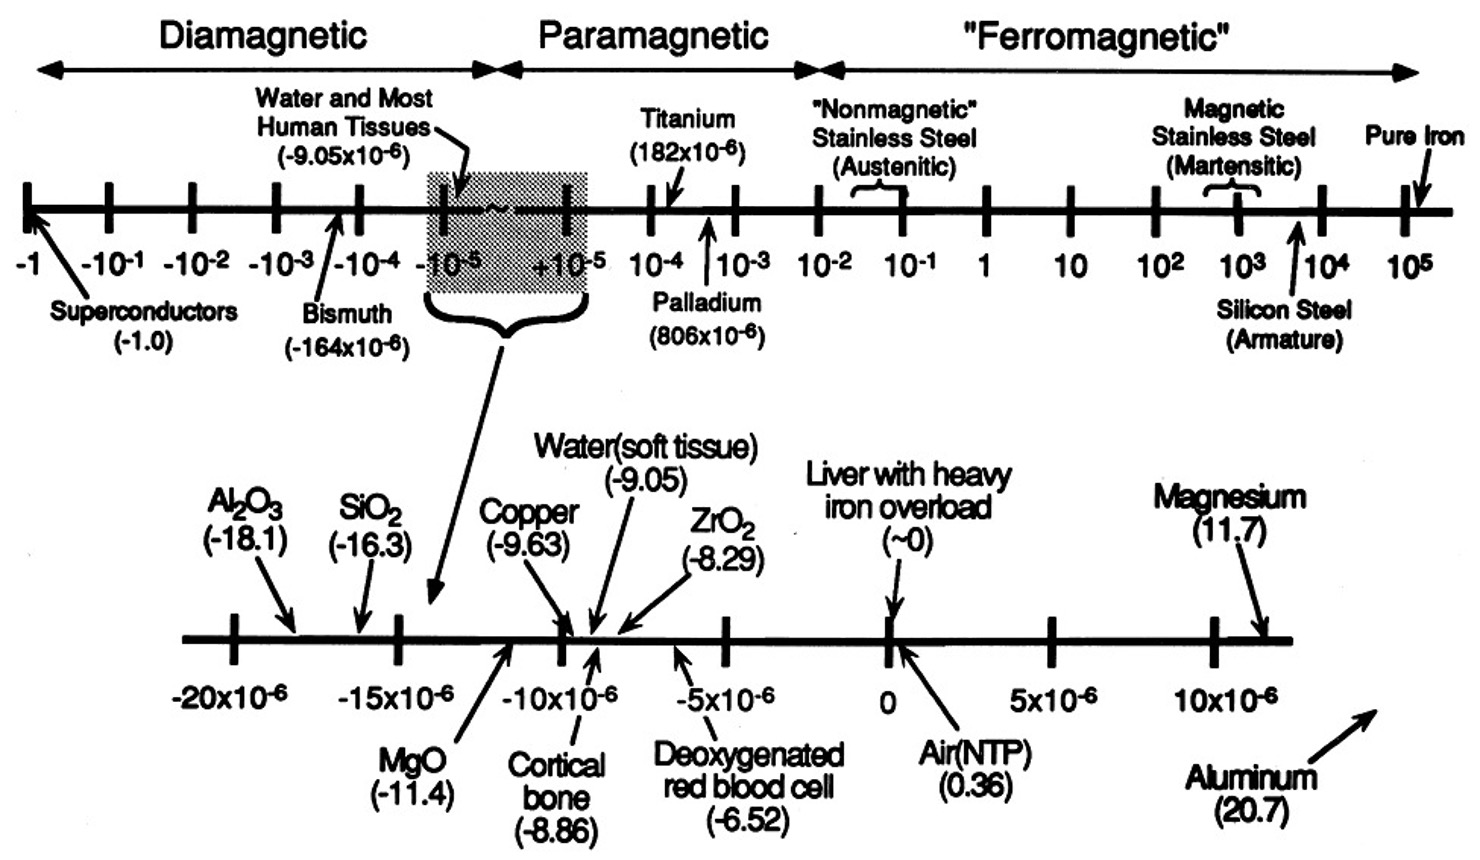
\includegraphics[width=0.95\textwidth]{Assets/Chi_inMRI.jpg}
%\caption[Spectrum of magnetic susceptibilities.]{
	%Spectrum of magnetic susceptibilities. The upper diagram uses a logarithmic scale to indicate the full range of observed magnetic susceptibility values, extending from -1.0 for superconductors to 100,000 for soft ferromagnetic materials. The bottom diagram uses a linear scale (in ppm) to indicate the properties of some materials with 20 ppm. The susceptibilities of most human tissues are in the range from -7.0 to -11.0 ppm. Adapted from Schenck \cite{Schenck2000}.}
%\label{fig:chi_spectrum}
%\end{figure}